\documentclass[authoryear]{elsarticle}

\usepackage{amsmath,amssymb}
\usepackage{mathtools}
\usepackage{tensor}
\usepackage{adjustbox}
\usepackage{multirow}
\usepackage{array}
\usepackage{threeparttable}
\usepackage[utf8]{inputenc}
\usepackage{booktabs, caption, makecell}
\usepackage{tikz}
\usetikzlibrary{arrows.meta,positioning,fit}
\usepackage[labelfont=bf]{caption} % Package to create caption to the figures

\usepackage{lineno,hyperref}
\modulolinenumbers[5]
\allowdisplaybreaks


% This avoid a foot note about to which paper the article was submited
\makeatletter
\def\ps@pprintTitle{%
 \let\@oddhead\@empty
 \let\@evenhead\@empty
 \def\@oddfoot{}%
 \let\@evenfoot\@oddfoot}
\makeatother

%%%%%%%%%%%%%%%%%%%%%%%
%% `Elsevier LaTeX' style
\bibliographystyle{plainnat}
%%%%%%%%%%%%%%%%%%%%%%%

\begin{document}

\begin{frontmatter}

\title{Centralized and decentralized logistics collaboration \\[5pt]
                \normalsize{Msc Thesis}}

%% Group authors per affiliation:
\author{Antón de la Fuente suárez-Pumariega}
\address{a.delafuentesuarez-pumariega@student.maastrichtuniverisry.nl }

%% or include affiliations in footnotes:
\author{Maastricht Univeristy}



\begin{abstract}
Here goes the abstract
\end{abstract}

\begin{keyword}
Here\sep go \sep KEY \sep words
\end{keyword}

\end{frontmatter}

% Desactivation of numbering every 15 LINES
%\linenumbers

\section{Introduction}

During the last decades, logistics collaboration, and specially \emph{horizontal
logistics collaboration}, has gained the attention of many researchers, as it
has been proofed to be an effective strategy to improve the logistics chain, for
example, reducing both ecological and economical 
costs \citep{BALLOT2010}, \citep{SOYSAL2018168}. By horizontal logistics collaboration we refer to the
cooperation between several companies or agents, who playing the same role in
the logistics chain, form coalitions or alliances to increase the efficiency of
their logistics operations. For example, in the case of the liner shipping
industry, by allowing other companies to use part of the capacity of the own
ships, increasing the asset utilization ratio \citep{AGARWAL2008175}.

When creating a new alliance, the involved companies have to agree which type of relation will define their collaboration. Among many others, to main elements have to be taken into consideration at this point: how much information they are willing to share with the other members of the coalition and how much decision power over their own strategies and operational plans they are willing to renounce to.

Different possibilities have been studied in the horizontal collaboration logistics literature. One of the types of collaboration most studied, representing around the 45\% of the works on the topic \citep{GANTERER2017}, is the one were agents share with a central authority all their information, to whom they also give all the power of decision. Known in the literature as \emph{central planning} systems, these cooperation mechanisms work aggregating all the assets and all the orders of the members of the coalition into a single bigger problem. That problem is solved using optimization techniques, to then share the benefits or the costs obtained with the cooperation among the members of the alliance. In the other hand, other cooperation mechanisms in which the agents only share part of their information with the central authority have also been studied. An example of these cooperation systems are the auction-based decentralized systems, where the members of the coalition first have to decide which information share with the others. For example, certain orders they cannot serve efficiently. Then the agents can announce their will to get assigned any of that shared orders. Finally a central authority, making use of auction techniques, decides how to allocate the shared orders among the interested agents \citep{VERDONCK2013}. 

Comparing the decentralized auction-based systems with the central planning ones, we observe that not only the amount of information shared by the agents differ, but also the degree of power decision given to the central authority. While in the central planning systems the individual agents only have to decide, and reach an agreement, about how to share the benefits of the cooperation, in the auction-based systems the agents not only decide which information to share with the others, but also how to serve the orders once they have been assigned to them. 

In this paper we explore different cooperation systems in the context of the horizontal logistics collaboration, with the intention of studying how the amount of information shared by the members of a coalition and the level of decision power they give to a central authority affects to the result of their collaboration. In section \ref{seq:litreview} we develop a review on the literature we have studied during the development of this work. In section \ref{seq:probdefinition} we define the problem we will use during the rest of this paper to illustrate the different systems we study and present the model for a single agent. Section \ref{seq:centrmodels} contains three different cooperation mechanisms which have in common the existence of a central authority with certain level of decision power. In section \ref{seq:itermodel} we introduce a, to best of our knowledge, novel approach to model a decentralized cooperative mechanism, were all the decision power remains in the agents, while the quantity of information they share is rather limited. Section \ref{seq:results} contains the results of the simulations we have done with the models presented in the two previous section. Section \ref{seq:discussion} is a discussion about the limitations and possible extensions of the models proposed in this paper. We finish with a conclusion in section \ref{seq:conclusion}.



\section{Literature review}\label{seq:litreview}

The literature studying the horizontal logistics collaboration between agents
can be divided in two main streams depending on whether the collaboration it is
centralized or not.

\subsection{Centralized cooperation}

In the case of centralized systems, agents share in a pool all or
part of the demands that they have to serve as well as the resources they have available. These resources can be vehicles in the case of transportation carriers, but also inventory levels, employees, etc. Then a central planner, taking into account all the demands and/or resources shared in the pool by the agents, solves the problem maximizing the total payoff of the coalition. Finally, the benefits of the cooperation are shared among the members of the coalition, usually using some allocation rule which ideally satisfies some desirable conditions in terms of ``fairness'', as that the resulting allocation is in the \emph{core}, i.e., any subcoalition of the former one could obtain a higher payoff working
independently \citep{GONZALEZ2010}. A well known example of an allocation rule fulfilling this conditions is the \emph{Shapley value} \citep{SHAPLEY1952}.

It has been pointed by \cite{DEFRYN2018891} that in the centralized planning systems, the individual objectives
of the agents are often not considered in favour of the coalition objective, what neglects the fact that the agents actually remain independent entities.  Accordingly with this idea,
these authors propose different mechanisms where both levels of objectives are
considered. In \cite{DEFRYN20191} a multiobjective approach were the members of a coalition can set up different objectives to the problem to be solved. In \cite{VANOVERMEIRE2014125} the allocation of the payoffs to each agent is integrated in the collaborative optimization problem, ensuring that the final solution accomplish certain predefined satisfaction level for all the agents. Furthermore, it is assumed
in the literature studying these type of systems that agents share all their private information
with the central planner, what might be unrealistic or problematic in real world cases \citep{SERRANO2017}, \citep{ZENG2015}.


\subsection{Decentralized cooperation}

In \cite{GANTERER2017} the decentralized cooperation systems are subdivided in two subclasses:  the ones based on auction and the rest. 

In the auction-based systems, the members of the coalition have to decide which of their orders they want to submit to a central pool, allowing the other members of the coalition to bid to be the ones serving that orders at some price. Then, a central planner, the auctioneer, has to resolve which bidder gets assigned which order shared in the pool. In \citep{PAN2019} two main problems that have to been solve during this process: first, the agents have to find which is their optimal bidding price for a request. In the other hand, the central authority has to solve how to allocate the orders to the agents, which is known as the winner determination problem. 

In the other hand,non-auction based decentralized systems have also been studied in the literature. In \cite{HERNANDEZ2014} a model where a single carrier can borrow at certain prices capacity to other collaborative carriers in a Less-than-truckload problem. Nevertheless, the model the authors proposed does not consider the possibility were multiple agents borrow and loan capacity at the same time. \cite{AGARWAL2008520}  propose a collaborative system based in a
inverse-optimization mechanism. The authors model a multicommodity flow problem, where agents own certain
fraction of the capacity of the edges of a network. The agents can collaborate sharing the capacity of the edges with the other members of the coalition, who have to pay some price for using that capacity. This mechanism requires that the agents share all the information with a central authority: how much capacity the agents own on each edge and which demands they have to serve.  Using inverse optimization, the prices at which agents exchange the capacity of their edges are decided by the central authority, in such a way that if the agents adopt that prices policy, when each
agent selfishly optimizes the flow of his demands through the network, the resulting flow will be the same that if a centralized planning approach was used. Therefore, even if full information is required and some decision power is left to a central planner, the decisions related on how to route the commodities and exchange resources are left to the agents. However, we argue that might be difficult or even unrealistic to implement in the real world a cooperation mechanism were a central authority with full information impose the prices at which the agents can exchange assets. In \cite{WANG2014} agents share orders in a common pool in a preprocessing stage. Then, a iterative process were agents propose routes to serve that orders and a central planner solves a winner determination problem to select the most efficient routes among the proposed ones is conducted. Once certain stop criteria is reached, a last winner determination problem is performed to find the final select routes, and the benefits, if any, of the cooperation are shared among the agents using some allocation rule.
In \cite{ANUPINDI2001} a novel framework to model decentralized systems is proposed. Based in the concept of \emph{coopetition} \citep{BRANDENBURGER1996},
the authors proposed a 2-stage mechanism to model the collaboration of agents in
decentralized distribution systems. In the first stage, agents individually
take strategic decisions, in their case, fixing their inventory levels. In the
seconds stage and after all the agents have served their demands in the best way they individually can, they cooperate sharing their residual demands and inventory with the others, obtaining extra profits. They propose sufficient conditions under which a Nash equilibrium in pure strategies exist for the first stage, and for which an allocation rule in the \emph{core} exists for the second stage.

None of the works above presented propose a cooperation system were no decision power at all is given to a central authority. A system with that characteristic, were all the decisions remain on the agents, is something that, to best of our knowledge, has not yet been studied in the current literature on horizontal logistics collaboration.


In this work we analyse and compare several cooperation systems, which differ on the degree of decision power and amount of information is left to a central planner. The first is a centralized planning system, were all information and decision are given to the central authority. The second and third systems we propose are based in a two stage process, which we borrow from \cite{ANUPINDI2001}. On these two systems, the agents start by, individually, making some decisions, after what they cooperate sharing certain information with a central authority which solves a centralized planning problem making use of that information. The last cooperation system we propose in this work is based in an iterative process of optimization and information sharing, which stops when the participants of the cooperation achieve an equilibrium point from which no agent would be interested to unilaterally deviate from. 

The problem we will use as example to implement these systems is a multicommodity flow problem, where each agent have to decide which edges to active on a network at certain price, to then find an efficient flow through them which maximizes their payoff. We select this problem because it captures both tactical and operational decision levels. In this way, we can study and compare the performance of models which differ on who, the agents or a central authority, is responsible of each level of decision making.

\section{Problem statement: A network design - multicommodity flow problem}\label{seq:probdefinition} 

The network design - multicommodity flow problem we propose in this work can be considered a 2-step problem, were an agent first make tactical decision, which edges to activate in a network, and after routes certain commodities through that network in a efficient way.
The objective of each agent is to maximize the revenues generated by his served commodities and minimize the costs associated with the activation of the edges.
The decision make in each step are intrinsically related: the most efficient flow an agent can find for his commodities depends on which edges he has activated, and to know which edges to activate, the agent need to know how he would route his commodities through any given set of active edges. 

We would model the scenario where the agents can collaborate among them sharing the capacity they do not use in their active edges, allowing others to route their commodities through them at some price. 

% On the rest of this section we will introduce the specific characteristics of these problem as well as the notation we will use. We will finish the section modelling the problem that each agent would face in case he does not take part of the collaboration.

Let $N=\{1,...,n\}$ be a set of agents. Let $G=(V,E)$ be a directed graph with
$V$ and $E$ the sets of nodes and edges respectively. 
Let $\Theta$ be the set of commodities. Each commodity $k$ has an origin node, $O(k)\in V$ and a destiny node, $T(k)\in V$, and is owner by the agent $W(k)\in N$. Every commodity $k$ has a size of $d_k$ units and has an associated revenue $r_k$ per unit. Thus, the owner of the commodity $k$ earns $d_k\cdot r_k$ if the commodity is successfully delivered from its origin to its terminal nodes. The commodities are unsplitable, i.e., cannot be divided between different edges. For each edge $e \in E$, we note as $O(e)\in V$ its origin node and by $T(e)\in V$ its terminal node. Furtheremore, $W(e)\in N$ is the owner of the edge $e\in E$. Note that could exist as many edges between a pair of nodes as agents in the coalition. Each edge $e \in E$ has certain units of capacity associated $q_e$, and a a fixed activation
cost $c_e$. This activation cost is the price the owner of the edge has to pay if he wants to use the edge to route any commodity. We will note by $\delta^+(v)\subset E$ the subset of edges whose origin is the node $v\in V$. Similarly, $\delta^-(v)\subset E$ is the subset of edges whose terminal node is $v\in V$. We will note by $E^i \subset E$ and $\Theta^i\subset \Theta$ the subsets of edges and commodities owned by agent $i$.

In table \ref{tb:notation} we summarize the notation we use during this work.

\begin{table}[ht!]
	\caption{Summary of notation \label{tb:notation}}
	\begin{tabular}{|l|l|}
	\hline
	Symbol & Meaning	 \\ \hline
	$N$ & Set of agents. \\
	$G$ & Network. \\
	$V$ & Set of nodes in $G$. \\
	$E$ & Set of edges in $G$. \\
	$\Theta$ & Sets of commodities. \\
	$\delta^+(v)$ & Subset of edges in $E$ which depart from node $v$.\\
	$\delta^-(v)$ & Subset of edges in $E$ which arrive to node $v$.\\	
	$\Theta^i$ & Set of commodities owned by agent $i$. \\	
	$E^i$ & Set of edges owned by agent $i$.\\
	$E_A$ & Subset of edges in $E$ that are active \\
	$E_R$ & Subset of edges in $E_A$ that have residual capacity.\\
	$k \in \Theta$ & A commodity\\
	$O(k)$ & Origin node of commodity $k$\\
	$T(k)$ & Destiny node of commodity $k$\\
	$W(k)$ & Agent who owns the commodity $k$\\
	$d_k$ & Size, on units, of commodity $k$.\\
	$r_k$ & Revenue, per unit, associated with serving commodity $k$.\\
	$e\in E$ & An edge\\
	$O(e)$ & Origin node of edge $e$\\
	$T(e)$ & Terminal node of edge $e$\\
	$W(e)$ & Agent who owns the edge $e$\\
	$c_e$ & Cost of activate edge $e$. \\
	$q_e$ & Units of capacity of edge $e$. \\
	$q_e^R$ & Units of residual capacity of edge $e$.\\
	\hline
	\end{tabular}
\end{table}

\subsection{Single agent model}

The objective of an agent $i \in N$ is to maximize his payoff, by routing his
commodities, $\Theta^i$, from their origin nodes to their terminal nodes through the edges, $E^i$, he has activated. Note that an agent does not have to necessarily serve all his commodities. In any case, it would be easy to extend the models presented in this work to fulfil that condition. Also we assume that an agent has always the possibility of activate one, and only one, edge between any two pair of nodes. In case we want to model a situation were some agents have not the possibility of activate certain edges, or limit the number of edges he can activate in total, we could simply make the capacity of certain edges equal to 0, or make their activation cost a very big number, making the activation of that edges not profitable under any circumstance. 

If the agent does not take part of the collaboration, she will not have any access to other agents' edges, neither the other agents can route their commodities through his edges. Thus, the problem which agent $i\in N$ has to solve can be modelled as the following ILP, that we call $P_i$,

    \begin{align}
        &  P_i: \quad \max  &  \sum_{k\in \Theta^i} \sum_{e \in \delta^+(T(k))\cap E^i} f_e^k \cdot d_k \cdot r_k - \sum_{e\in E^i} u_e\cdot c_e \hspace{20pt} &&   \label{eq:SingleAgentA}
    \end{align}
    \begin{align}
        & \text{subject to:}       &  \nonumber\\
       & \sum_{e \in \delta^-(z)\cap E^i} f_e^k-\sum_{e \in \delta^+(z)\cap E^i} f_e^k = 0,\quad && \forall\ z\in V\setminus\{O(k),T(k)\},\ \forall\ k\in\Theta^i,  \label{eq:SingleAgentB}\\
        &    \sum_{e \in \delta^+(T(k))\cap E^i} f_e^k \leq 1,  && \forall\ k\in \Theta^i, \label{eq:SingleAgentC} \\
		& \sum_{e \in \delta^+(T(k))\cap E^i} f_e^k= 0,  && \forall\ k\in \Theta^i, \label{eq:SingleAgentD} \\
		& \sum_{k \in \Theta^i} f_e^k \cdot d_k \leq u_e\cdot q_e, && \forall\ e \in E^i,\label{eq:SingleAgentE}  \\
		& \sum_{\substack{e \in E^i\colon \\ O(e),T(e) \in S}} f_e^k \leq |S| -1,   && \forall\ S \subset V,\ \forall\ k \in \Theta^i, \label{eq:SingleAgentF}\\[1em]
		& f_e^k \in \{0,1\},    && \forall\ e \in E^i,\ \forall\ k \in \Theta^i, \label{eq:SingleAgentG} \\ 
		&  u_e   \in \{0,1\},           && \forall\ e \in E^i 
    \end{align}

where, $\forall\ k\in \Theta^i$ and  $\forall\ e \in E$,
\[
\begin{array}{rl}
f_e^k = & \begin{cases}
    1 & \text{if } k \text{ is routed through } e,\\
    0 & \text{otherwise}
\end{cases}  \\[20pt]
u_e = &\begin{cases}
    1 & \text{if } e \text{ is active},\\
    0 & \text{otherwise}    
\end{cases}
\end{array}
\]

The objective of agent $i$, equation (\ref{eq:SingleAgentA}), is to maximize the
profit generated by the commodities which arrive to their destination nodes
while minimizing the cost associated to the activation of the edges. Constraints
(\ref{eq:SingleAgentB}) ensure that, for any commodity, the flow that enters
and leaves every transit nodes (neither the origin, neither the terminal node of
that commodity) is equal. Constraints (\ref{eq:SingleAgentC}), together with
(\ref{eq:SingleAgentG}), guarantee that each commodity is send at most only once
from its origin node. Constraints (\ref{eq:SingleAgentD}) ensure that no
commodity is send from its terminal node to any other node. Constraints (\ref{eq:SingleAgentE})
ensure that the capacity of edges is not exceed. Finally, constraints
(\ref{eq:SingleAgentF}) are subtour elimination constraints \citep{AHUJA1993}. 

%We have included it in our model because, first of all, it makes sense to assume that an agent would not want to create subtours when routing his commodities. Note that subtours could be possible without this constraint because once an edge is activated, there is no extra costs for routing more commodities through it. Furthermore, without the subtour elimination constraints, the other constraints are not sufficient to ensure that all the feasible solution of the ILP are admissible, since the flow of a commodity could contain a subtour disconneted from the origin and terminal nodes of that commodity, without impacting the objective but making the solution not valid for the problem we are modelling.

In a simplifying abuse of notation, we will refer with $P_i^*$ both to the value of the objective function for the optimal solution of $P_i$ as well as to the values of the decision variables have in that optimal solution. For instance, we can say that the edge $e\in E^i$ is active in the optimal solution of $P_i$ if $u_e=1$ in $P_i^*$. At the same time, we say that $P_i^*$ is the maximum payoff agent $i$ can obtain without collaborating with other agents.

\section{Three cooperation models with a central authority with decision power} \label{seq:centrmodels}

In the previous subsection, we have presented an ILP that models the network design - multicommodity flow problem of an agent $i\in N$ who works alone. In this section, we present different cooperative systems, where the agents in $N$ collaborate in different ways in order to find synergies among them and increase their payoffs.

The three models we propose in these section follow the same structure, composed of two stages. In the first stage, every agent $i\in N$ solves its own problem without cooperating with the others, $P_i$, and shares with a central authority some information based in the optimal solution he has found (which information is exactly shared depends on the model). In the second stage the central authority solves the cooperative problem, which is different in each of the three models, as it depends in the amount of information the edges has shared and in the degree of power decision they have give to him. In figure \ref{fig:generalflowchart} we present the general structure of these systems.


\begin{figure}[ht!]
\centering
\caption{Structure of the three models where the central authority has some decision power \label{fig:generalflowchart}}
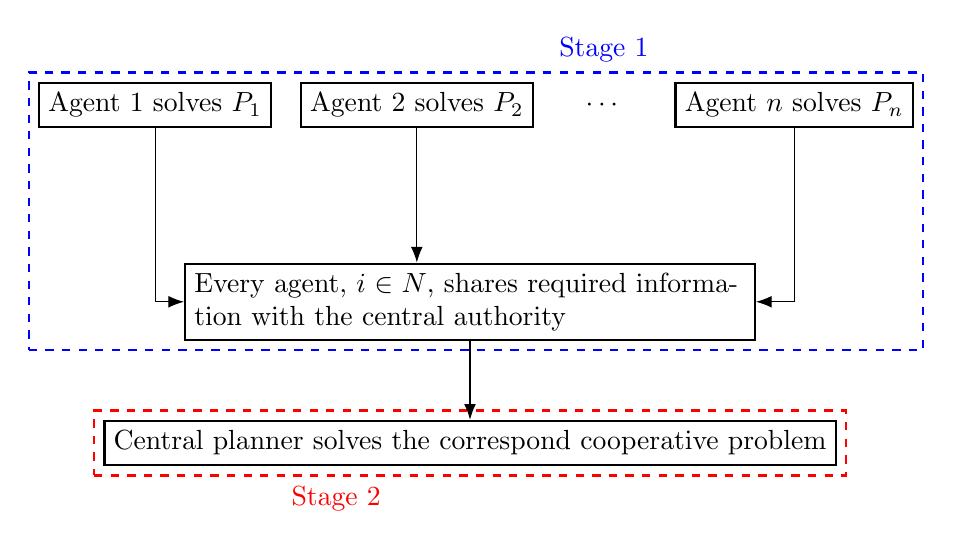
\begin{tikzpicture}
	\begin{scope}[every node/.style={rectangle,draw,thick,minimum height=16pt,minimum width =30pt}]
		\node[draw=none,blue] (Stage1) at (1.7,0.7) {Stage 1}	;
		\node (A1) at (-4,0) {Agent 1 solves $P_1$};
		\node[right =10pt of A1] (A2) {Agent 2 solves $P_2$};
		\node[draw=none,right =10pt of A2] (pass) {$\cdots$ };
		\node[right =10pt of pass] (An) {Agent $n$ solves $P_n$};
		\node[align = left,text width=7cm] (shares) at (0,-2.5) {Every agent, $i\in N$,  shares required information with the  central authority};
    		\node[below = of shares] (central) {Central planner solves the correspond cooperative problem};
    		\node[draw=none,red] (Stage2) at (-1.7,-5) {Stage 2}	;

    		
    		\node [fit=(A1) (An) (shares),draw,dashed,thick,blue] {};
 		\node [fit=(central) ,draw,dashed,thick,red] {};

	\end{scope}
	
	\begin{scope}
	\draw[-{Latex[length=2mm]}] (A1.south) |- (shares.west);
	\draw[-{Latex[length=2mm]}] (A2) edge (A2.south|-shares.north);
	\draw[-{Latex[length=2mm]}] (An.south) |- (shares.east);
	\draw[-{Latex[length=2mm]}] (shares) edge (central);

	\end{scope}
\end{tikzpicture}
\end{figure}

In table \ref{tb:summarycentralizedmodels} we summarize which decisions are left to the central authority and which are left to the agents in each model. The \emph{full cooperation system} assumes that full information is shared with the central authority, and all the decision power is given to him. In the \emph{partial cooperation system}, agents decide in the first stage which edges to activate and inform about their decisions and all the information about the commodities they have to serve to the central authority. Then, the central authority find the most efficient flow of all the commodities through the edges the agents have activated. Finally, in the \emph{residual cooperation system}, agents first decide which edge to activate and route their commodities through them maximizing their individual payoffs. Then they share with the central planner the commodities they have not served as well as their active edges which still have some unused capacity. Then, in the second stage the central planner tries to route the shared commodities using the available capacity in the shared edges.


\begin{table}[ht!]
	\centering
	\caption{Summary of decision making allocation between agents and central authority \label{tb:summarycentralizedmodels}}
    \begin{threeparttable}
        \begin{tabular}{p{0.2\textwidth}>{\centering}p{0.19\textwidth}>{\centering}p{0.15\textwidth}>{\centering}p{0.1\textwidth}>{\centering\arraybackslash}p{0.15\textwidth}}
            & &      \multicolumn{3}{c}{Coop. systems with a central authority} \\\cline{3-5}
            & & Centralized &  Partial & Residual \\ \hline
            \multirow{2}{*}{Agents} & Activate edges & No & Yes & Yes \\
            & Route flow     & No & No & Yes \\\hline
            \multirow{2}{*}{Central authority} & Activate edges & Yes & No & No \\
            & Route flow & Yes & Yes & Yes\tnote{*} \\\bottomrule
        \end{tabular}
    \begin{tablenotes}\footnotesize
        \item[*] Only the residual commodities through the residual capacities
        of the active edges.
        \end{tablenotes}
    \end{threeparttable}
    \end {table}

We have already state that the way in which agents can collaborate with each other is by sharing the capacity of the edges they have activated with other agents at some price. This might allow some agents to serve commodities in a more efficient way with respect to the non-cooperative scenario, and generate extra profit to the owner of the edges which are used by other agents.
We assume that the the revenues generated by the cooperation are allocate following the next rules:
\begin{enumerate}
    \item The revenues generated by any served commodity are
    allocated to its owner.
    \item The activation cost of any active edge is paid by its owner.
    \item If a commodity $k\in \Theta$ is routed through an edge $e		\in E$ and $W(k)\not = W(e)$, the agent who owns the commodity, $W(k)$ makes a side payment equal to $d_k \cdot\frac{c_e}{q_e}$ to the agent who owns the edge, $W(e)$. In words, for each commodity sent through an edge owned by other agent, the owner of the commodity will pay to the owner of the edge the fraction of the activation cost of that edge equivalent 	to the fraction of the total capacity of the edge that his 	commodity occupies.\footnote{The models could easily be adapted to allow the agents to individually choose the prices at which other agents can use capacity of their edges.}
\end{enumerate}

In the rest of this section we introduce the three different
cooperative systems with a central authority with decision power we propose in this work.


\subsection{Fully centralized cooperation system}

We start introducing the model where more power is given to the central planner.
In this model, the agents start by solving their individual problems in the non-cooperating scenario, $P_i\  \forall i \in N$. Then they share all their commodities and edges the central authority. Each agent also inform to the central planner about which is the maximum payoff they can obtain without cooperating. In the second stage the central authority solves a new ILP, $\Gamma_F$, which is almost identical to $P_ i$, the ILP that an agent $i\in N$ has to solve when no cooperating. Both problems only differ in
two aspects (see \ref{seq:appendixilp} for a complete overview of the ILP):

\begin{enumerate}[(a)]
	\item The central planner manages the commodities and edges of
all the agents, $\Theta$ and $E$, while without cooperation an agent $i$ only has access to his own commodities and edges, $\Theta^i$ and $E^i$.
	\item The following two new constraints are added to the problem:

\begin{equation}
\sum_{e \in \delta^-(T(k))}  f_e^k \cdot d_k \cdot r_k - \sum_{\substack{e \in E^j\colon \\ j\not = i}} f_e^k \cdot d_k \cdot \frac{c_e}{q_e}\geq 0,  \forall\ k \in \Theta, \label{eq:commodirevenue}
\end{equation}
\begin{equation}
\varphi_i(\Gamma_F) \geq P_i^*,  \forall\ i\in N; \label{eq:newconstraintFullCooperation}
\end{equation}

Constraints (\ref{eq:commodirevenue}) avoids that the central planner serves a commodity in such a way that the side payments his owner has to make are higher than the revenue he obtains for serving that commodity. Furtheremore, with constraints (\ref{eq:newconstraintFullCooperation}), similarly to the idea introduced by \cite{VANOVERMEIRE2014125}, we integrate the final payoffs of the agents, $\varphi_i$ for each $i \in N$, in the constraints of the central planner's problem. Thus, these constraints  ensure that the final payoff of every agent is greater or equal than what that agent could achieve without cooperation, i.e., $P_i^*$.  Doing so we can say that the final payoff allocation is \emph{individually rational} \citep{GONZALEZ2010}, i.e., no single agent is interested in leaving the coalition unilaterally.  \footnote{We can extend this idea by forcing the solution resulting from the cooperation to be in the \emph{core}, by adding constraints ensuring that any the sum of the payoffs of the members of any subcoalition is equal or greater than what that agents could obtain by leaving the grand coalition and cooperating only among them. Nevertheless, doing it will increase the complexity of the models and we consider that it does not add value to the paper.}

For each agent $i\in N$, we define its final payoff as

\begin{equation}
    \begin{split}
    & \varphi_i(\Gamma_F) =\label{eq:FullCooperationPayoff} \\
    & = \sum_{(o,t,i)\in \Theta^i} \left[ \sum_{e \in \delta^-(t)\cap E^i} f_e^{(o,t,i)} \cdot d_{(o,t,i)} \cdot r_{(o,t,i)} -  \sum_{\substack{e\in \Theta^j \colon\\ j\not = i}} f_e^{(o,t,i)} \cdot d_{(o,t,i)} \cdot \frac{c_e}{q_e} \right]  \\
    & + \sum_{\substack{(o,t,k) \in \Theta  \colon \\ k \not = i}} \left[\sum_{e \in E^i} f_e^{(o,t,k)} \cdot d_{(o,t,k)} \cdot \frac{c_e}{q_e}\right] - \sum_{e \in E^i} u_e \cdot c_e, 
    \end{split}
\end{equation}

\end{enumerate}


The first term of equation (\ref{eq:FullCooperationPayoff}) is the sum of the profit associated with the commodities of the agent, which for each commodity is equal to the revenue it
generates when it is served minus the cost the agent has to pay to other agents if the commodity passes through edges which does not belong to him. The second sum is the payments that other agents make to him when routing their commodities through his edges. The last term is the sum of the costs of the active edges.

In figure \ref{fig:centralizedmodel} we present a flowchart with the structure of this model.


\begin{figure}[ht!]
\centering
\caption{Flowchart of the centralized partial cooperation system \label{fig:centralizedmodel}}
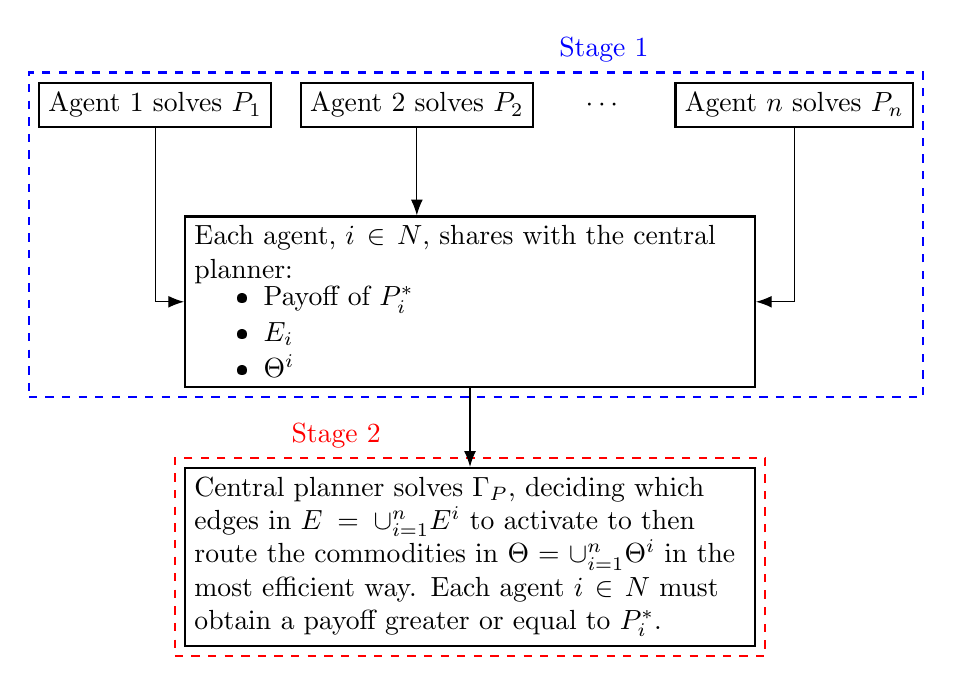
\begin{tikzpicture}
	\begin{scope}[every node/.style={rectangle,draw,thick,minimum height=16pt,minimum width =30pt}]
		\node (A1) at (-4,0) {Agent 1 solves $P_1$};
		\node[right =10pt of A1] (A2) {Agent 2 solves $P_2$};
		\node[draw=none,right =10pt of A2] (pass) {$\cdots$ };
		\node[right =10pt of pass] (An) {Agent $n$ solves $P_n$};
		\node[align = left,text width=7cm] (shares) at (0,-2.5) {Each agent, $i\in N$,  shares with  the  central planner:\vspace{-10pt}
		\begin{itemize}
			\itemsep-3pt 
        		\item Payoff of $P_i^*$
        		\item $E_i$ 
        		\item $\Theta^i$
   		 \end{itemize}
    };
    \node[below = of shares,align = left,text width=7cm] (central) {Central planner solves $\Gamma_P$, deciding which edges in $E=\cup_{i=1}^n E^i$ to activate to then route the commodities in $\Theta=\cup_{i=1}^n \Theta^i$ in the most efficient way. Each agent $i\in N$ must obtain a payoff greater or equal to $P_i^*$.};
    
    \node [fit=(A1) (An) (shares),draw,dashed,thick,blue] {};
    \node[draw=none,blue] (Stage1) at (1.7,0.7) {Stage 1}	;
 	\node [fit=(central) ,draw,dashed,thick,red] {};
 	\node[draw=none,red] (Stage2) at (-1.7,-4.2) {Stage 2}	;
	\end{scope}
	
	\begin{scope}
	\draw[-{Latex[length=2mm]}] (A1.south) |- (shares.west);
	\draw[-{Latex[length=2mm]}] (A2) edge (A2.south|-shares.north);
	\draw[-{Latex[length=2mm]}] (An.south) |- (shares.east);
	\draw[-{Latex[length=2mm]}] (shares) edge (central);

	\end{scope}
\end{tikzpicture}
\end{figure}

\subsection{Central routing cooperation system}

In the centralized routing cooperation system, the central authority has to optimize once again the flow of all the commodities of all the agents through the network, maximizing the total generated revenue. Nevertheless, the decision of which edges to activate remains as an individual decision of each agent.


\begin{figure}[ht!]
\centering
\caption{Flowchart of the central routing cooperation system \label{fig:partialmodel}}
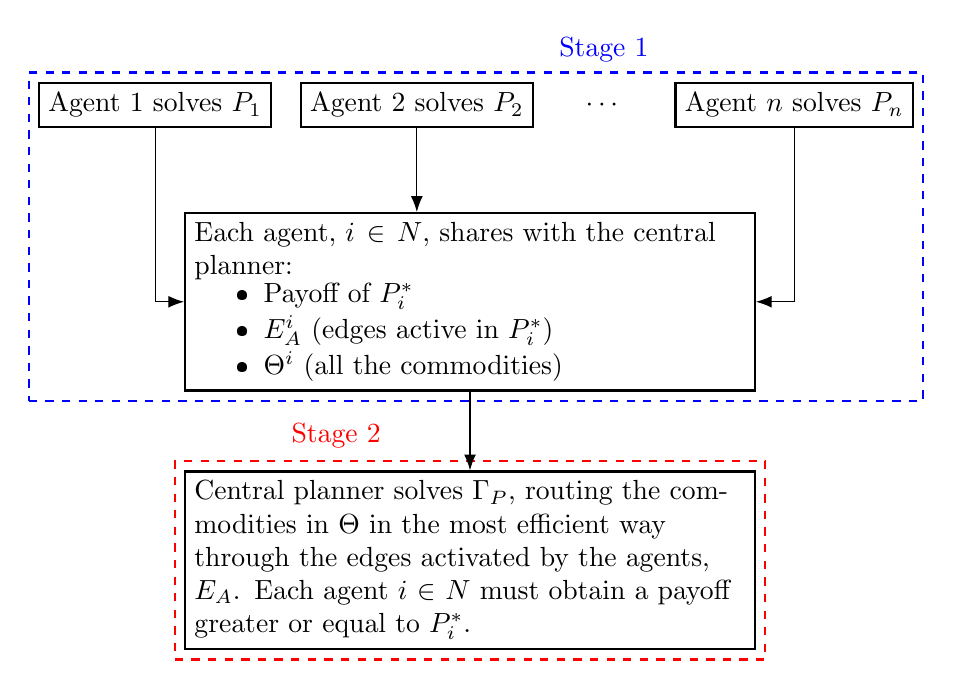
\begin{tikzpicture}
	\begin{scope}[every node/.style={rectangle,draw,thick,minimum height=16pt,minimum width =30pt}]
		\node (A1) at (-4,0) {Agent 1 solves $P_1$};
		\node[right =10pt of A1] (A2) {Agent 2 solves $P_2$};
		\node[draw=none,right =10pt of A2] (pass) {$\cdots$ };
		\node[right =10pt of pass] (An) {Agent $n$ solves $P_n$};
		\node[align = left,text width=7cm] (shares) at (0,-2.5) {Each agent, $i\in N$,  shares with  the  central planner:\vspace{-10pt}
		\begin{itemize}
			\itemsep-3pt 
        		\item Payoff of $P_i^*$
        		\item $E_A^i$ (edges active in $P_i^*$)
        		\item $\Theta^i$ (all the commodities)
   		 \end{itemize}
    };
    \node[below = of shares,align = left,text width=7cm] (central) {Central planner solves $\Gamma_P$, routing the commodities in $\Theta$ in the most efficient way through the edges activated by the agents, $E_A$. Each agent $i\in N$ must obtain a payoff greater or equal to $P_i^*$.};
    
    \node [fit=(A1) (An) (shares),draw,dashed,thick,blue] {};
    \node[draw=none,blue] (Stage1) at (1.7,0.7) {Stage 1}	;
 	\node [fit=(central) ,draw,dashed,thick,red] {};
 	\node[draw=none,red] (Stage2) at (-1.7,-4.2) {Stage 2}	;
	
	\end{scope}
	
	\begin{scope}
	\draw[-{Latex[length=2mm]}] (A1.south) |- (shares.west);
	\draw[-{Latex[length=2mm]}] (A2) edge (A2.south|-shares.north);
	\draw[-{Latex[length=2mm]}] (An.south) |- (shares.east);
	\draw[-{Latex[length=2mm]}] (shares) edge (central);

	\end{scope}
\end{tikzpicture}
\end{figure}

In the first stage, every agent $i \in N$ solves his own $P_i$ problem. Then, each agent $i\in N$, shares with the central authority all his commodities, $\Theta^i$, and inform him about which is the maximum payoff he can obtain without cooperating, $P_ i^*$ and which edges he would activate in that case, $E_A^i$. In the second stage, the central authority solves a new ILP, $\Gamma_P$, routing all the commodities of all the agents, $\Theta=\cup_{i=1}^n \Theta^i$, through all the edges agents would have activated in the non-cooperation scenario, $E_A=\cup_{i=1}^n E_A^i$, and ensuring no agent $i\in N$ get a payoff lower than $P_i^*$. In figure \ref{fig:partialmodel} we present a flowchart summarizing these steps.

Therefore the ILP, $\Gamma_P$, that the central planner has to solve in this \emph{central routing cooperation system} is

\begin{align}
        &  \Gamma_P: \max  & \sum_{k \in \Theta} \sum_{e \in \delta^-(T(k))\cap E_A}  f_e^k \cdot d_k \cdot r_k  &&   \label{eq:PartialCooperationA} 
    \end{align}
    \begin{align}
        & \text{subject to:}       && \nonumber\\
        & \sum_{e \in \delta^-(z)\cap E_A} f_e^k-\sum_{e \in \delta^+(z)\cap E_A} f_{e}^k = 0,            \quad && \forall\ z\in V\setminus\{O(k),T(k)\},\ \forall\ k\in\Theta,  \label{eq:PartialCooperationB}\\[1em]
& \sum_{e \in \delta^+(O(k))\cap E_A} f_e^k \leq 1,  && \forall\ k\in \Theta, \label{eq:PartialCooperationC} \\
& \sum_{e \in \delta^+(T(k))\cap E_A} f_e^k = 0,  && \forall\ k\in \Theta, \label{eq:PartialCooperationD} \\
 & \sum_{k \in \Theta} f_e^k\cdot d_k \leq q_e     && \forall\ e \in E_A, \label{eq:PartialCooperationE}  \\
 & \sum_{\substack{e \in E_A\colon \\ O(e),T(e) \in S}} f_e^k  \leq |S| -1,    && \forall\ S \subset V,\ \forall\ k \in \Theta, \label{eq:PartialCooperationF}\\
&\sum_{e \in \delta^-(T(k))\cap E_A}  f_e^k \cdot d_k \cdot r_k 
 -\sum_{\substack{e \in E_A^j\colon \\ j\not = i}} f_e^k \cdot d_k \cdot \frac{c_e}{q_e}\geq 0, && \forall\ k \in \Theta, \label{eq:PartialCooperationG} \\
& \varphi_i(\Gamma_P)   \geq P_i^*,     && \forall\ i\in N \label{eq:PartialCooperationH}\\
 & f_e^k  \in \{0,1\},    && \forall\ e \in E_A, \forall\ k \in \Theta, \label{eq:PartialCooperationI}
    \end{align}

Note that, this model differs from the previously presented in this work in the absence of decisions variables for the activation of the edges, since this decision is previously make by the agents and not left to the central planner. Also, as in the \emph{full cooperation system}, we include the constraints (\ref{eq:PartialCooperationG}) and (\ref{eq:PartialCooperationH})
which are equivalent to the constraints (\ref{eq:commodirevenue}) and (\ref{eq:newconstraintFullCooperation}). In this case, because the absence of the decision variables $u_e$ in the model, we redefine the payoff allocate to each agent $i\in N$ as follows

\begin{equation}
    \begin{split}
    & \varphi_i(\Gamma_P) =\label{eq:PartialCooperationPayoff} \\
    & = \sum_{(o,t,i)\in \Theta^i} \left[ \sum_{e \in \delta^-(t)\cap E_A} f_e^{(o,t,i)} \cdot d_{(o,t,i)} \cdot r_{(o,t,i)} -  \sum_{\substack{e\in E^j \colon\\ j\not = i}} f_e^{(o,t,i)} \cdot d_{(o,t,i)} \cdot \frac{c_e}{q_e} \right] + \\
    & + \sum_{\substack{(o,t,k) \in \Theta  \colon \\ k \not = i}} \left[\sum_{e \in E_A^i} f_e^{(o,t,k)} \cdot d_{(o,t,k)} \cdot \frac{c_e}{q_e}\right] - \sum_{e \in E_A^i} c_e.
    \end{split}
\end{equation}

\subsection{Central residuals routing cooperation system}

In this system, the agents would once again start by solving their individual problems, $P_i$ for each $i\in N$. Nevertheless, this time the agents  would actually implement the optimal solution they found for this problems, $P_i^*$ for each $i\in N$. Then, they would inform the central authority about which commodities they were not able to serve when working alone, $\Theta_R^i$, as well as which edges they have activated still have some residual capacity $E_R^i$. In the second stage, the central authority routes the residual commodities of all the agents $\Theta_R = \cup_{i=1}^n \Theta_R^i$ through the edges with residual capacity, $E_R=\cup_{i=1}^n E_R^i$. Furtheremore, the sum of the sizes of the commodities the central planner route through an edge $e\in E_R$ cannot exceed the residual capacity, which we note by $q_e^R$, that the owner of that edge, $W(e)\in N$, has left unused after implementing $P_{(W(e)}^*$.


\begin{figure}[ht!]
\centering
\caption{Flowchart of the centralized residual cooperation system \label{fig:residualmodel}}
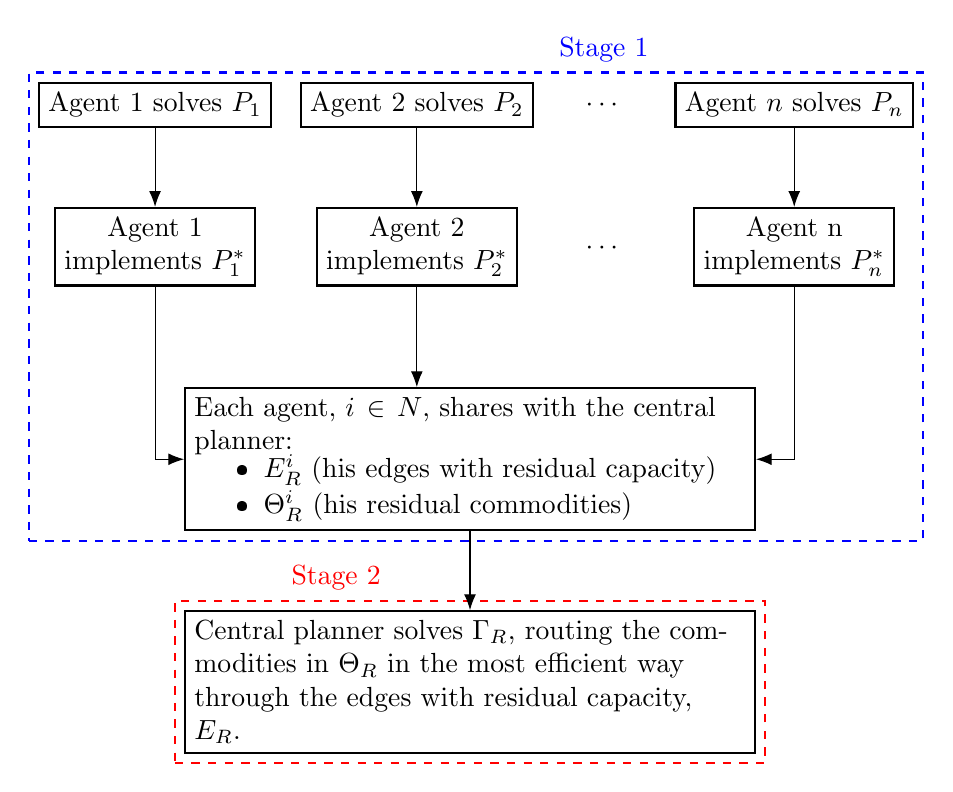
\begin{tikzpicture}
	\begin{scope}[every node/.style={rectangle,draw,thick,minimum height=16pt,minimum width =30pt}]
		\node (A1) at (-4,0) {Agent 1 solves $P_1$};
		\node[right =10pt of A1] (A2) {Agent 2 solves $P_2$};
		\node[draw=none,right =10pt of A2] (pass) {$\cdots$ };
		\node[right =10pt of pass] (An) {Agent $n$ solves $P_n$};
		\node[below = of A1,align = center] (A1impl) {Agent 1 \\ implements $P_1^*$};
		\node[below = of A2,align = center] (A2impl) {Agent 2 \\ implements $P_2^*$};
		\node[draw=none,below =35pt of pass] (pass2) {$\cdots$ };
		\node[below = of An,align = center] (Animpl) {Agent n \\ implements $P_n^*$};
		\node[align = left,text width=7cm] (shares) at (0,-4.5){Each agent, $i\in N$,  shares with  the  central planner:\vspace{-10pt}
		\begin{itemize}
			\itemsep-3pt
        		\item $E_R^i$ (his edges with residual capacity)
        		\item $\Theta_R^i$ (his residual commodities)
   		 \end{itemize}
    };
    \node[below = of shares,align = left,text width=7cm] (central) {Central planner solves $\Gamma_R$, routing the commodities in $\Theta_R$ in the most efficient way through the edges with residual capacity, $E_R$.};
    
	  \node [fit=(A1) (An) (shares),draw,dashed,thick,blue] {};
    \node[draw=none,blue] (Stage1) at (1.7,0.7) {Stage 1}	;
 	\node [fit=(central) ,draw,dashed,thick,red] {};
 	\node[draw=none,red] (Stage2) at (-1.7,-6) {Stage 2}	;    
    
	\end{scope}
	
	\begin{scope}
	\draw[-{Latex[length=2mm]}] (A1) edge (A1impl);
	\draw[-{Latex[length=2mm]}] (A2) edge (A2impl);
	\draw[-{Latex[length=2mm]}] (An) edge (Animpl);
	\draw[-{Latex[length=2mm]}] (A1impl.south) |- (shares.west);
	\draw[-{Latex[length=2mm]}] (A2impl) edge (A2.south|-shares.north);
	\draw[-{Latex[length=2mm]}] (Animpl.south) |- (shares.east);
	\draw[-{Latex[length=2mm]}] (shares) edge (central);

	\end{scope}
\end{tikzpicture}
\end{figure}

The ILP the central planner has to solve in this central residuals routing cooperation system, $\Gamma_R$, is equivalent to $\Gamma_P$, where the commodities and edges the central planner manages are $\Theta_R$ and $E_R$ instead of $\Theta$ and $E_A$. Also, as the central planner cannot route commodities through an edge $e\in E_R$ exceeding the residual capacity of that edge, $q_e^R$, the constraints (\ref{eq:PartialCooperationE}) are substituted by

\begin{equation}
\sum_{k \in \Theta_R} f_e^k\cdot d_k \leq q_e^R,\quad \forall\ e \in E_R.
\end{equation}
in this ILP. See \ref{seq:appendixilp} for a full overview of this ILP.
    
In this system, it is guaranteed by design that each agent receives  payoff greater or equal than the payoff they could obtain by their own, as they always first implement the best solution they can achieve without cooperating, and therefore they can only increase their payoffs with respect to that value. Therefore, constraints equivalent to (\ref{eq:PartialCooperationH}) are not included. Under the residual cooperation system we define the final payoff of an agent $i\in N$ as

\begin{equation}
    \begin{split}
    & \varphi_i(\Gamma_R) =\label{eq:ResidualCooperationPayoff} \\
    & = \sum_{k\in \Theta^i_R} \left[ \sum_{e \in \delta^-(T(k))\cap E_R} f_e^k \cdot d_k \cdot r_k -  \sum_{\substack{e\in E^j_R \colon\\ j\not = i}} f_e^k \cdot d_k \cdot \frac{c_e}{q_e} \right] + \\
    & + \sum_{\substack{k \in \Theta_R  \colon \\ W(k) \not = i}} \left[\sum_{e \in E_R^i} f_e^k \cdot d_k \cdot \frac{c_e}{q_e}\right] - P_i^*
    \end{split}
\end{equation}


\section{A fully decentralized cooperation mechanism for two agents} \label{seq:itermodel}

In this section we propose a fully decentralized cooperation mechanism for two agents, where all the decisions are left to the agents, who make use of an \emph{information platform} to interact with each other.

The idea behind this mechanism is that the agents exchange information in an iterative process, informing to the other agent about the residual capacity they have in their own active edges, allowing the other agent to use that residual capacity to route his commodities at some price.

Before going in more detail about how the cooperation mechanism works, we introduce how the information platform works. Each agent $i\in N$ has two different ``pools" to share information:

\begin{description}
	\item[Shared edges:] Agent $i$ can share a subset of his active edges which still have some residual capacity, $\widehat{E}_R^i\subseteq E_R^i$. He also has to share how many units of residual capacity has each edge $e\in \widehat{E}_R^i$, $q_e^R$, and which is the cost of each of that units, $\frac{c_e}{q_e}$
	\item[Demanded edges:] If agent $j$ has previously shared a set of edges in the platform, agent $i$ can make use those edges when routing his commodities. If agent $i$ actually decides to route a subset of his commodities, $\widehat{\Theta}^i\subset \Theta ^i$ through some of that edges, he has to share in the information platform:
	\begin{enumerate}
		\item How much units of capacity he requires (or demands) in total on each edge $e$ shared by agent $j$, what we note by $q_e^D$.
	\item For each commodity $k\in \widehat{\Theta}^i$, a set $L^k$, containing the edges shared by agent $j$ through which the commodity would be routed. Also which would be the side payment he would make to agent $j$ if finally all the edges $e$ in $L^k$ are active and he can make use of $q_e^D$ units of capacity in each of them. That side payment is computed as $p_{L^k}=\sum_{e \in L^k} d_k\cdot \frac{c_e}{q_e}$. We note by $\mathcal{L}^i$ the set containing all $L^k,\ \forall\ k \in \widehat{\Theta}^i$.
	\end{enumerate}
		
\end{description}	

Making use of the information platform just introduced, both agents iteratively solve an ILP. In each iteration both agents, sequentially and not in parallel, decide which edges to activate, and how to route their commodities through the network, as they do in $P_i$, but this time, they can route their commodities, through the edges shared in the platform by the other agent with the corresponding costs and respecting the available capacities on that edges. Furthermore, when deciding if activate or not an edge, each agent does not only have to account for the activation cost, but also for the side payments the other agent is willing to make to him if he activates certain combinations of edges and leaves on them certain residual capacities. The ILP, $\Upsilon_i$, agent $i\in N$ has to solve in each iteration is the following:

    \begin{align}
        &  \Upsilon_i: \hspace{10pt} \max  &&  \sum_{k\in \Theta^i} \sum_{e \in \delta^-(T(k))\cap (E^i\cup \widehat{E}_R^j)} f_e^k \cdot d_k \cdot r_k - \sum_{e\in E^i} u_e\cdot c_e \hspace{20pt} -  \nonumber  \label{eq:IterativeA}\\
        & 								  && - \sum_{k \in \Theta^i} \sum_{\substack{e \in \widehat{E}_R^j\colon \\ j\not = i}} f_e^k \cdot d_k \cdot \frac{c_e}{q_e}   + \sum_{\substack{L^k \in \mathcal{L}^j \colon \\ W(k)\not = i}} p_{L^k} \cdot t_{L^k}
    \end{align}
    \begin{align}
        & \text{subject to:}       && \nonumber\\
& \sum_{e \in \delta^-(z)\cap (E^i\cup \widehat{E}_R^j)} f_e^k-\sum_{e \in \delta^+(z)\cap (E^i\cup \widehat{E}_R^j)} f_{e}^k  = 0,                                   && \forall\ z\in V\setminus\{O(k),T(k)\},\nonumber\\[-1em]
& && \forall\ k\in\Theta^i,  \label{eq:IterativeB}\\[1em]
& \sum_{e \in \delta^+(O(k))\cap (E^i\cup \widehat{E}_R^j)} f_e^k  \leq 1, && \forall\ k\in \Theta^i, \label{eq:IterativeC} \\
& \sum_{e \in \delta^+(T(k))\cap (E^i\cup \widehat{E}_R^j)} f_e^k  = 0,  && \forall\ k\in \Theta^i, \label{eq:IterativeD} \\
& \sum_{k \in \Theta^i} f_e^k\cdot d_k \leq u_e\cdot q_e, && \forall\ e \in E^i, \label{eq:IterativeE}  \\
& \sum_{k \in \Theta^i} f_e^k\cdot d_k \leq  q_e^R, && \forall\ e \in \widehat{E}_R^j,\label{eq:IterativeF}  \\
& \sum_{\substack{e \in E^i\cup \widehat{E}_R^j\colon \\ O(e),T(e) \in S}}  f_e^k  \leq |S| -1, && \forall\ S \subset V,\ \forall\ k \in \Theta^i, \label{eq:IterativeG}\\
&\sum_{k\in \Theta^i} f_e^k \cdot d_k \leq (q_e - q_e^D) +M(1-b_e),\quad && \forall e \in L^{\bar{k}},\nonumber\\[-5pt]
& && \forall L^{\bar{k}} \in \mathcal{L}^j, \label{eq:IterativeH}\\[5pt]
&b_e \leq u_e, && \forall e\in L^k,\nonumber\\[-5pt]
& && \forall L^k \in \mathcal{L}^j, \label{eq:IterativeI}\\[5pt]
& t_{L^k} \leq 1 -  (|L^k|-\sum_{e \in L^k} b_e), && \forall L^k \in \mathcal{L}^j \label{eq:IterativeJ}\\
& f_e^k  \in \{0,1\}, && \forall\ e \in E^i,\ \forall\ k \in \Theta^i, \label{eq:IterativeK} \\
&  u_e   \in \{0,1\},   && \forall\ e \in E^i,  \label{eq:IterativeL}\\
& b_e \in \{0,1\}, && \forall e \in L^k,\ \forall L_k\in \mathcal{L}^j,\label{eq:IterativeM}\\[5pt]
& t_{L^k} \in \{0,1\}, && \forall L^k \in \mathcal{L}^j, \label{eq:IterativeN}
    \end{align}
where $M$ is a very large value.

In $\Upsilon_i$, the first term of the objective function of the agent $i$, equation (\ref{eq:IterativeA}), is the sum of the revenue generated by the commodities which are served. The second term is the sum of the costs of the edges he has activate. The third term is the sum of the side payments he has to do when routing commodities through the edges shared by the other agent. Finally, the fourth term is the sum of the side payments he receives from the other agent for making use of the edges he has shared in the previous iteration, if they remain available in the conditions the other agent has demanded.

Constraints (\ref{eq:IterativeB}), (\ref{eq:IterativeC}), (\ref{eq:IterativeD}) and (\ref{eq:IterativeG}) are equivalent to constraints (\ref{eq:SingleAgentB}),(\ref{eq:SingleAgentC}),(\ref{eq:SingleAgentD}) and (\ref{eq:SingleAgentF}) in $P_i$, with the difference that now the agent $i$ can use the edges shared in the information platform by the agent $j$, $\widehat{E}_R^j$. Constraint (\ref{eq:IterativeE}) is identical to constraint (\ref{eq:SingleAgentE}) and constraint (\ref{eq:IterativeF}) is an extension of it, ensuring that the agent does not exceed the residual capacity of the edges shared by agent $j$ when routing his commodities.

Constraints (\ref{eq:IterativeH}),  (\ref{eq:IterativeI}) and (\ref{eq:IterativeJ}) together with the ``technical" decision variables (\ref{eq:IterativeM}) and (\ref{eq:IterativeN}), are related with the side payments agent $i$ receives from agent $j$. Recall that each $L^k \in \mathcal{L}^j$ is a set which contains the edges of agent $i$ that agent $j$ has indicated in the previous iteration he would like to use to route commodity $k$. He has also indicates that if and only if for every $e \in L^k$, $q_e^R$ units of capacity are available to him, he would make a side payment to agent $i$ equal to $p_{L^k}$. Thus, in order to get the side payment $p_{L^k}$, the technical decision variable $t_{L^k}$ must be equal to 1. Constraints (\ref{eq:IterativeJ}) and (\ref{eq:IterativeN}) ensures that $t_{L^k}$ only can be 1 if all the technical decision variables $b_e$ for $e \in L^k$ are also equal to 1. Finally, constraints (\ref{eq:IterativeH})  making use of the \emph{big M} coefficient, and (\ref{eq:IterativeI}), ensures that if $b_e$ is equal to one, agent $i$ must leave at least $q_e^D$ units of residual capacity on that edge and the edge $e$ must be active. Note that these constraints are too restrictive. Agent $j$ might be planning to route 2 or more commodities through the edge $e$, and even if agent $i$ left less than $q_e^R$ units of capacity available, he might be possible to route, not all, but some of that commodities through it. However, these constraint assume that none of the commodities could be routed and therefore, any side payment associated with a commodity passing through that edge would be done. We argue that capture with exactitude this behaviour would make the model too complex, as the problem of deciding which commodities can still be routed and which cannot is a \emph{knapsack problem}, which has been proven to be NP-complete \citep{KARP1972}.

In figure \ref{fig:iterflowchart} we present a flow chart illustrating the structure of these cooperation mechanism.
In the first iteration, as the information platform is empty, agent 1 is in practice solving $P^1$. Indeed, if the no information was shared in the platform, $\Upsilon^i=P^i$. For the same reason, in the first iteration agent 2 does not expect any side payments from agent 1 (he have not got yet the opportunity of demanding any edges, since no edges were shared for agent 2 in the platform yet). The iterative process continues until an equilibrium is found or the maximum number of iteration allowed is reached or an equilibrium is found. We define an \emph{equilibrium} as the situation were the solutions of $\Upsilon^1$ and $\Upsilon^2$ found in the iteration $h$ are exactly the same than the solutions found in the iteration $h-1$. This is equivalent to the definition of the \emph{Nash equilibrum}: given the actions of the others, an agent cannot individually improve their payoff by changing his strategy \citep{GONZALEZ2010}. If the maximum number of iteration is reached without equilibrium, the mechanism considers that no solution was found.


\begin{figure}[ht!]
\centering
\caption{Flowchart of the decentralized cooperation mechanism for two agents\label{fig:iterflowchart}}
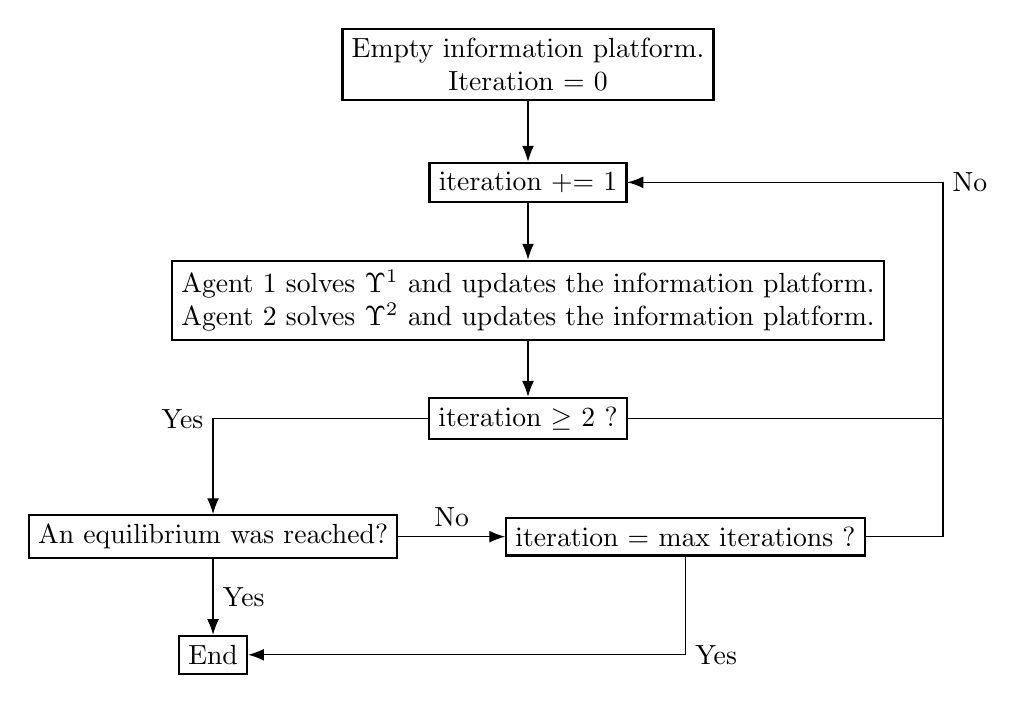
\begin{tikzpicture}
\begin{scope}[every node/.style={rectangle,draw,thick}]
	\node[align = center] (init) at (0,0)  {Empty information platform.\\
	Iteration = 0};
	\node (iteration) at (0,-1.5){iteration += 1};
	\node[align =left] (main) at (0,-3) {Agent 1 solves $\Upsilon^1$  and updates the information platform.\\
	Agent 2 solves $\Upsilon^2$  and updates the information platform.};
	\node (itquestion) at (0,-4.5) {iteration $\geq$ 2 ?};

	\node (equiquestion) at (-4,-6) {An equilibrium was reached?};

	\node (maxit) at (2,-6) {iteration = max iterations ?};

	\node (End) at (-4,-7.5) {End};
\end{scope}

\begin{scope}
	\draw[-{Latex[length=2mm]}] (init) edge (iteration);
	\draw[-{Latex[length=2mm]}] (iteration) edge (main);
	\draw[-{Latex[length=2mm]}] (main) edge (itquestion);
	\draw[-{Latex[length=2mm]}] (itquestion.east)  -- ++(4cm,0) |- node[right] {No}
	 (iteration.east);
	\draw[-{Latex[length=2mm]}] (itquestion.west) -| node[left] {Yes} (equiquestion);
	\draw[-{Latex[length=2mm]}] (equiquestion)  edge node[above] {No} (maxit);
	\draw[-{Latex[length=2mm]}] (equiquestion) edge node[right] {Yes} (End);
	\draw[-{Latex[length=2mm]}] (maxit.south) |- node[right] {Yes} (End);
	\draw[-] (maxit.east)  -- ++(0.98cm,0) |- (iteration.east);




\end{scope}

\end{tikzpicture}
\end{figure}

\section{Results} \label{seq:results}

In order to analyse the performance of the different models discussed in the work, we tested the 4 different cooperation mechanism over 20 instances of the network design - multicommodity flow problem introduced in section \ref{seq:probdefinition}, comparing them with the no cooperation system, by simply solving the single agent model (presented also in section \ref{seq:probdefinition}) and summing the payoff of all the agents.

The models were implemented in Python 3.8 and solved using CPLEX 20.1, by means of the DOCplex library. The tests were performed in an  Intel(R) Core(TM) i7-5500U CPU @ 2.40GHz with 8GB of RAM.

Both the instances and the code are available upon request.


\subsection{Instance generation}

We have created 20 instances for the network design - multicommodity flow problem introduced in section \ref{seq:probdefinition}. We have decided to randomly generate them and not to use them for two main reasons. First of all, we could not found on the Internet any set of test instances matching exactly our problem characteristics. Secondly, we found sets of test instances for multicommodity flow problems \citep{MCFPWEB} and we considered to adapt them to our problem. Nevertheless, all this instances were too big, and since we are using an exact ILP solver we considered that to use very complex instances was not appropriate for this work.

Therefore, we randomly generate 20 instances, all sharing the following characteristic: a complete and directed graph $G(V,E)$ with 7 nodes, ($|V|=7$), is generated. For each edge $e\in E$, we randomly select its activation cost, $c_e$, from a uniform distribution $U[3,6]$. Also for each commodity $(o,t,i)\in \Theta$ we randomly select its size and revenue per unit from two uniform distributions, $U[0,5]$ and $U[1,2]$ respectively. Finally, we differentiate 4 classes among the 20 problem cases, each containing 5 instances, which differ in the number of agents and the capacity of the edges considered. Two of the four classes consider cases with 2 agents, and the other two, with 5. At the same time, among the two instances with the same number of agents,  in one class the capacity of the edges is randomly selected from a uniform distribution $U[2,8]$ (LOW capacity), and for the other class from a uniform distribution $U[5,12]$ (HIGH capacity).
The name of each instance indicates to which class they belong: for example, the instance ``\texttt{2\_LOW\_0}'' has 2 agents and the capacities of the edges were selected from the $U[2,8]$ distribution. The last number is just a index to differentiate the five instances inside the same class (from 0 to 4).

\subsection{Parameter selection}

Only in the decentralize iterative cooperation mechanism there is a parameter, and only one, which is the maximum number of iterations allowed. In our test we set it equal to 100. Furthermore, we have also model this mechanism in our simulations in such a way that the agents always share all their edges with residual capacity in the information platform, i.e., $\widehat{E}_R^i=E_R^i\ \forall\ i\in N$.

\subsection{Comparision 3 centralized mechanisms}

In table [REF!] we presented the results of the three different centralized models tested over the 10 instances with 5 agents. Each cell represents the sum of the final payoffs (total payoffs) of all the agents. The first column corresponds to the no cooperation system, were the agents do not collaborate at all. Columns 2,4 and 6 corresponds to the total payoffs for the full, partial and residual cooperation systems, and columns 3,5,7 to the percentage of improvement of each of that cooperation systems with respect to the no cooperation case.

Furtheremore, in table [REF!] the running times of each mechanism are reported. We want to remark that this running times must be taken as references and not exactly values. This is because for the 3 centralized systems, the computations of the best solution of each agent when no cooperating were performed sequentially and not in parallel. It could be argued that in a real word case, each agent would make these computations by his own, at least in the residual cooperation system, where the central planner does not need to have access to all the information of each agent, neither to check if the payoff they have reported as the best they can obtain without cooperation is true (as it does not take part of the constraints).

\subsection{Comparision centralized mechanisms and iterative one, all for 2 agents}
 

In this subsection we present the results for the instances where only 2 agents are involved. 

First of all, in table \ref{tb:iter_order_comparition} we compare the total payoffs obtained from the decentralized iterative cooperation mechanism depending on which agent goes first in the iterative process. The first two columns are the total payoff associated to each of the two possible orders, and the third column the percentage of difference between the two. The number of iterations required to reach an equilibrium in each case are presented in columns 3 and 4, and column 5 is the difference on number of iterations required between both orders.



\begin{table}[ht!]
\centering
\caption{Analysis of the impact of the order of the agents in the iterative mechanism \label{tb:iter_order_comparition}}
\begin{adjustbox}{max width=\textwidth}
\begin{tabular}{lrrrrrr}
\toprule
{} &  Order1\_payoff &  Order2\_payoff &      Dif\% &  Order1\_it &  Order2\_it &  Dif\_it \\
\midrule
2\_low\_0  &           25.0 &           25.0 &  0.00 &        4.0 &        3.0 &     1.0 \\
2\_low\_1  &           21.0 &           21.0 &  0.00 &        3.0 &        3.0 &     0.0 \\
2\_low\_2  &           17.0 &           17.0 &  0.00 &        3.0 &        3.0 &     0.0 \\
2\_low\_3  &           15.0 &           15.0 &  0.00 &        4.0 &        4.0 &     0.0 \\
2\_low\_4  &           27.0 &           26.0 &  3.70 &        3.0 &        3.0 &     0.0 \\
2\_high\_0 &           73.0 &           72.0 &  1.37 &        3.0 &        3.0 &     0.0 \\
2\_high\_1 &           70.0 &           69.0 &  1.49 &        3.0 &        3.0 &     0.0 \\
2\_high\_2 &           65.0 &           63.0 &  3.08 &        3.0 &        3.0 &     0.0 \\
2\_high\_3 &           68.0 &           67.0 &  1.47 &        4.0 &        4.0 &     0.0 \\
2\_high\_4 &           74.0 &           73.0 &  1.35 &        3.0 &        3.0 &     0.0 \\
\bottomrule
\end{tabular}
\end{adjustbox}
\end{table}


Tables \ref{tb:2_payoffs}, and \ref{tb:2_times} are equivalent to tables [REF!], and [REF!] with the difference that the decentralized iterative cooperation mechanism is now included. For this mechanism, we have reported in table \ref{tb:2_payoffs} the lower total payoff among the two possible ones, depending in the order in which the agents participate on it, i.e., for each instance the minimum among the values in colum 1 and 2 of table \ref{tb:iter_order_comparition}

\begin{table}[h!]
\centering
\caption{Comparision of the payoff obtained by each cooperative mechanism for instances with two agents \label{tb:2_payoffs}}
\begin{adjustbox}{max width=\textwidth}
\begin{tabular}{lrrrrrrrrr}
\toprule
{} &  No coop &   Full &   \% &  Partial &  \% &  Residual &  \% &  Iterative &  \% \\
\midrule
2\_low\_0  &            22.0 &   47.0 &  113.64 &     35.0 &     59.09 &      22.0 &       0.00 &       25.0 &       13.64 \\
2\_low\_1  &            19.0 &   43.0 &  126.32 &     29.0 &     52.63 &      20.0 &       5.26 &       21.0 &       10.53 \\
2\_low\_2  &            15.0 &   39.0 &  160.00 &     29.0 &     93.33 &      17.0 &      13.33 &       17.0 &       13.33 \\
2\_low\_3  &            11.0 &   34.0 &  209.09 &     19.0 &     72.73 &      11.0 &       0.00 &       15.0 &       36.36 \\
2\_low\_4  &            23.0 &   45.0 &   95.65 &     30.0 &     30.43 &      25.0 &       8.70 &       26.0 &       13.04 \\
2\_high\_0 &            69.0 &  100.0 &   44.93 &     82.0 &     18.84 &      69.0 &       0.00 &       72.0 &        4.35 \\
2\_high\_1 &            67.0 &  105.0 &   56.72 &     83.0 &     23.88 &      67.0 &       0.00 &       69.0 &        2.89 \\
2\_high\_2 &            61.0 &   92.0 &   50.82 &     71.0 &     16.39 &      63.0 &       3.28 &       62.0 &        1.64 \\
2\_high\_3 &            62.0 &   97.0 &   56.45 &     77.0 &     24.19 &      63.0 &       1.61 &       67.0 &        8.06 \\
2\_high\_4 &            70.0 &  105.0 &   50.00 &     83.0 &     18.57 &      72.0 &       2.86 &       73.0 &        4.29 \\
\bottomrule
\end{tabular}
\end{adjustbox}
\end{table}

\begin{table}[h!]
\centering
\caption{Comparision of the running times of each cooperative mechanism for instances with two agents\label{tb:2_times}}
\begin{tabular}{lrrrrr}
\toprule
{} &     Full &  Partial &  Residual &  Iterative \\
\midrule
2\_low\_0  &               9.85 &     3.74 &      2.44 &       6.12 \\
2\_low\_1  &                 9.45 &     2.96 &      2.45 &       6.45 \\
2\_low\_2  &                6.32 &     2.49 &      2.13 &       3.47 \\
2\_low\_3  &                 5.16 &     2.37 &      2.12 &       5.37 \\
2\_low\_4  &                 5.23 &     3.48 &      2.85 &       4.86 \\
2\_high\_0 &             1088.24 &    61.73 &     60.51 &     237.08 \\
2\_high\_1 &              415.45 &    46.60 &     41.79 &     152.41 \\
2\_high\_2 &              221.80 &    56.95 &     55.29 &     137.38 \\
2\_high\_3 &              241.28 &    62.92 &     60.02 &     130.08 \\
2\_high\_4 &              174.32 &    49.51 &     45.84 &      59.72 \\
\bottomrule
\end{tabular}
\end{table}





\section{Discussion} \label{seq:discussion}

In this section we comment different aspects about the mechanism we have studied in this work as well as the results we have obtained with the simulations, as well as possible extensions for them and open questions for future research.

\subsection{Results discussion}


Table \ref{tb:2_payoffs} show us how the decentralized iterative cooperation mechanism cannot compete with the full and partial cooperation systems in terms of total payoffs. Furthermore, the partial cooperation systems is also faster in terms of running time. In the other hand, this mechanism is able to find better solutions than the residual cooperation system in nine of the ten instances in exchange for slightly longer running times. Having into account that the among of information agents require to share in the decentralized mechanism is less than in the centralized residual system, were agents share their residual edges but also their residual commodities and leave the routing decisions to the central planner, we consider argue that if the running times are not a limitation, the decentralized iterative system is superior to the centralized residual cooperation system. \footnote{Of course, the decentralized system is only comparable with the centralized ones when only 2 agents are involved in the problem.}

We can observe in table \ref{tb:iter_order_comparition} that even if the order of the agents does not appear to affect in general to the number of iteration necessary to reach an equilibrium (with the exception of instance ``\texttt{2\_LOW\_0}"), it can have an impact in the total payoff obtained. This seems specially relevant in the instances were the capacity of the edges is higher. A first hypothesis to justify this could be that, as already stated before, a higher capacity in the edges of the graph could mean a bigger number of possibilities to cooperate, making the order in which the agents participate in the process more relevant. Nevertheless, the number of iterations necessary to reach an equilibrium does not grows with the capacity of the edges, and therefore more experiments would be necessary in order to find a reason for this behaviour. 

Another interesting results is that an equilibrium was always found in the 10 studied instances, and that the number of iterations required to find is is relatively constant, varying between 3 and 4 iterations in all the cases.
\subsection{Possible extensions and future work}

Several extensions can be done in order to make this work more complete. Probably the most obvious is to extend the decentralized iterative cooperation mechanism to more than 2 agents. Nevertheless, a direct extension could derive in requiring more iterations in order to reach an equilibrium, or even making that equilibrium unlikely to exist. Also, might be possible that if the number of agents increases, the relevance of the order in which that agents participate in the iterative process increases too. In any case, more work is required in order to confirm or not the above hypothesis.

Another possibility we considered and finally we did not include in this work because of time limitations, is to study a version of the 
decentralized iterative cooperation mechanism where the agents cannot change their decision, both respect to the design of their network neither the flow of their commodities, if they have already share information in the platform related with them. For example, if an agent has shared an edge with residual capacity in the previous iteration and the other agent has requested to use it, he would not be allowed to change his mind and deactivate it in future iterations. We hypothesize that this could reduce the number of iterations required  to reach an equilibrium and maybe make the extension to more than 2 agents easier. In the other hand,a system like this could generate less quality solutions from the point of view of the whole coalition and increase the relevance of the order in which the agents participate in the iterative process. Once again, more work and further experiments are necessary to can confirm these hypothesis.

In the other hand, the centralized cooperation systems proposed in this work could be also improved. For example, in the partial cooperation systems, the agents might follow different or even better strategies for deciding which edges to activate than simply solve their individuals optimization problem, $P^i$ for $i\in N$, and choosing the edges that are activate in the respective solutions. Also, more constraints could be added to the three centralized cooperation models, in order to make the solutions not only individually rational, but to force them to be in the core. Other open question is which solution should selected in case that exist multiple optimal solutions for the problem that the central planner has to solve in any of these three mechanism. For instance, multiobjectives approaches could be investigated.


\section{Conclusion} \label{seq:conclusion}

In this work we have proposed three difference centralized cooperation systems and a, to the best of our knowledge, novel decentralized cooperation system for two agents. We have model these systems to solve a network design - multicommodity flow problem. Then we have simulate a set of instances to test our models, finding that the decentralized systems is only competitive with the centralized system were the central planner has less decision power, and outperformed by the other two. Nevertheless, the small amount of information agents need to share in the decentralized system might be a reason to dedicate future work to extend it to more than two agents, as well as study different variations of it. 

\bibliography{bibliography}

\appendix
\section{ILP's}
\label{seq:appendixilp}

\subsection{ILP to be solved by the central planner in the fully centralized cooperation system.}

    \begin{align}
        &  \Gamma_F: \max  & \hspace{22pt} \sum_{k\in \Theta} \sum_{e \in \delta^-(T(k))\cap E}  f_e^k \cdot d_k \cdot r_k - \sum_{e\in E} u_{e}\cdot c_{e} \hspace{40pt} && 
    \end{align}
    \begin{align}
        & \text{subject to:}       && \nonumber \\
        & \sum_{e \in \delta^-(z)\cap E} f_e^k -\sum_{e \in \delta^+(z)\cap E} f_{e}^k = 0,\quad && \forall\ z\in V\setminus\{O(k),T(k)\},\ \forall\ k\in\Theta, \\
& \sum_{e \in \delta^+(O(k))\cap E} f_e^k \leq 1, && \forall\ k\in \Theta, \\
 & \sum_{e \in \delta^+(T(k))\cap E} f_e^k = 0,  && \forall\ k\in \Theta,  \\
& \sum_{k \in \Theta} f_e^k\cdot d_k  \leq u_e\cdot q_e, && \forall\ e \in E,   \\
 & \sum_{\substack{e \in E\colon \\ O(e),T(e) \in S}} f_e^k \leq |S| -1, && \forall\ S \subset V,\ \forall\ k \in \Theta,\\
&\sum_{e \in \delta^-(T(k))\cap E}  f_e^k  \cdot d_k \cdot r_k - \sum_{\substack{e \in E^j\colon \\ j\not = i}} f_e^k \cdot d_k \cdot \frac{c_e}{q_e}\geq 0, && \forall\ k \in \Theta, \\
& \varphi_i(\Gamma_F) \geq P_i^*,  && \forall\ i\in N, \\
& f_e^k \in \{0,1\},  && \forall\ e \in E,\ \forall\ k \in \Theta,  \\
&  u_e  \in \{0,1\},  && \forall\ e \in E.
   \end{align}

\subsection{ILP to be solved by the central planner in the central  residuals routing cooperation system.}

  \begin{align}
        &  \Gamma_R: \max  & \sum_{k \in \Theta_R} \sum_{e \in \delta^-(T(k))\cap E_R}  f_e^k \cdot d_k \cdot r_k &&   
    \end{align}
    \begin{align}
        & \text{subject to:}       && \nonumber\\
        & \sum_{e \in \delta^-(z)\cap E_R} f_e^k-\sum_{e \in \delta^+(z)\cap E_R} f_{e}^k  = 0,           \quad && \forall\ z\in V\setminus\{O(k),T(k)\},\ \forall\ k\in\Theta_R, \\[1em]
& \sum_{e \in \delta^+(O(k))\cap E_R} f_e^k\leq 1, && \forall\ k\in \Theta_R,  \\
& \sum_{e \in \delta^+(T(k))\cap E_R} f_e^k  = 0, && \forall\ k\in \Theta_R,  \\
 & \sum_{k \in \Theta_R} f_e^k\cdot d_k \leq q_e^R   &&\forall\ e \in E_R,   \\
& \sum_{\substack{e\in E_R\colon\\O(e),T(e)\in S }} f_e^k \leq |S| -1,  && \forall\ S \subset V, \ \forall\ k \in \Theta_R, \\
& \sum_{e \in \delta^-(T(k))\cap E_R}  f_e^k  \cdot d_k \cdot r_k -\sum_{\substack{e \in E_R^j\colon \\ j\not = i}} f_e^k \cdot d_k \cdot \frac{c_e}{q_e}\geq 0, && \forall\ k \in \Theta_R, \\
& f_e^k \in \{0,1\},    && \forall\ e \in E_R, \forall\ k \in \Theta_R.
    \end{align}

\end{document}